\section{Compilers in general}

New programming languages are often developed to allow for a higher level of abstraction and a higher level of reasoning about algorithms. To be able to run these new languages, compilers are built to convert the high level code either down to machine code, to run directly on hardware, or to an intermediate language to make use of already existing compilers.

\begin{figure}[!ht]
  \centering
  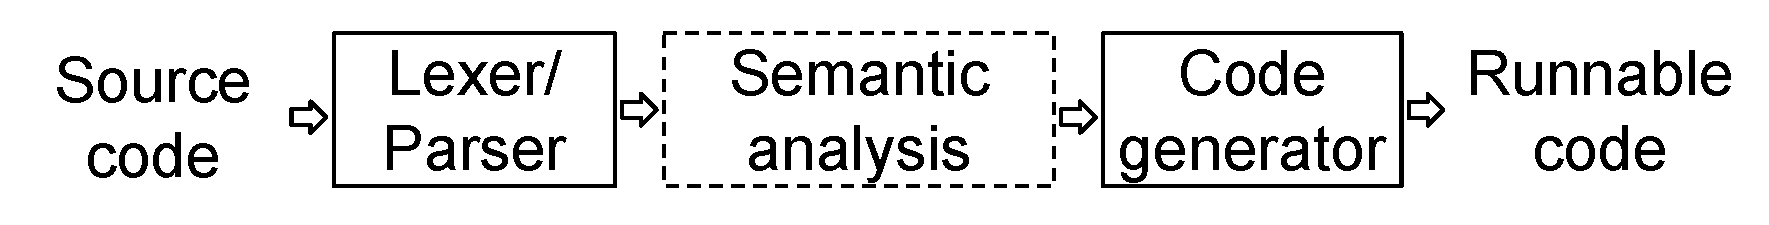
\includegraphics[width=0.6\pdfpagewidth]{figure/generalpipeline}
  \caption{A general compiler pipeline}
  \label{fig:generalpipeline}
\end{figure}

The structure of a compiler can be likened to a pipe where text flows through. The text flowing through the pipe is transformed between different representations, and is in the end output as runnable code to either run on the computer itself or on a virtual machine that emulates a computer. 

To ensure that the compiled program is correct and does what it is intended to do, \gls{seman} is performed upon the code. An example of such analysis is building a call graph to identify unreachable code and to make sure that variables are defined before use. Another example is \gls{typechecking}, where type correctness is proved, which is used heavily in Haskell.

Figure~\ref{fig:generalpipeline} shows the flow handling of the source code. It should be noted that \gls{seman} is optional: languages may rely entirely on the grammar as their only way to expose errors. This will lead to a more expressive, or less restricted, language, but increases the risk of runtime crashes due to type errors.

The next section continues by describing the first step of the compilation process, lexing and parsing.
